% Diagrama de secuencia — Pronóstico de demanda con AMS (estado 2026-09)
\documentclass[tikz, border=14pt]{standalone}
\usepackage[utf8]{inputenc}
\usepackage[T1]{fontenc}
\usepackage{helvet}
\renewcommand{\familydefault}{\sfdefault}
\usetikzlibrary{arrows.meta}

\tikzset{
  arr/.style={line width=0.8pt, -{Latex[length=2.3mm]}},
  ret/.style={line width=0.8pt, dashed, -{Latex[length=2.3mm]}},
  lbl/.style={font=\footnotesize\sffamily, fill=white, inner sep=1.2pt, align=center},
  head/.style={draw, line width=0.8pt, fill=black!12, minimum width=3.4cm, minimum height=0.9cm,
    align=center, font=\small\sffamily\bfseries},
}
% \msg{x origen}{x destino}{y}{texto}  ·  \ret igual, punteado  ·  \self{x}{y}{texto}
\newcommand{\msg}[4]{\draw[arr] (#1,#3) -- (#2,#3) node[midway, above, lbl] {#4};}
\newcommand{\ret}[4]{\draw[ret] (#1,#3) -- (#2,#3) node[midway, above, lbl] {#4};}
\newcommand{\self}[3]{\draw[arr] (#1,#2) -- ++(0.5,0) -- ++(0,-0.4) -- ++(-0.5,0);
  \node[lbl, anchor=west, align=left] at (#1+0.6,#2-0.2) {#3};}
% \frag{x1}{y1}{x2}{y2}{operador}{guarda}
\newcommand{\frag}[6]{\draw[line width=0.7pt] (#1,#2) rectangle (#3,#4);
  \draw[line width=0.7pt, fill=white] (#1,#2) -- ++(1.0,0) -- ++(0,-0.3) -- ++(-0.15,-0.2) -- (#1,#2-0.5) -- cycle;
  \node[font=\footnotesize\sffamily\bfseries] at (#1+0.45,#2-0.25) {#5};
  \node[font=\footnotesize\sffamily, anchor=west] at (#1+1.1,#2-0.25) {#6};}
\newcommand{\els}[4]{\draw[line width=0.7pt, dashed] (#1,#2) -- (#3,#2);
  \node[font=\footnotesize\sffamily, anchor=west, fill=white, inner sep=1.5pt] at (#1+0.1,#2-0.25) {#4};}

\def\xU{0} \def\xA{4.2} \def\xB{8.8} \def\xS{13.4} \def\xM{18.0} \def\xD{22.6}

\begin{document}
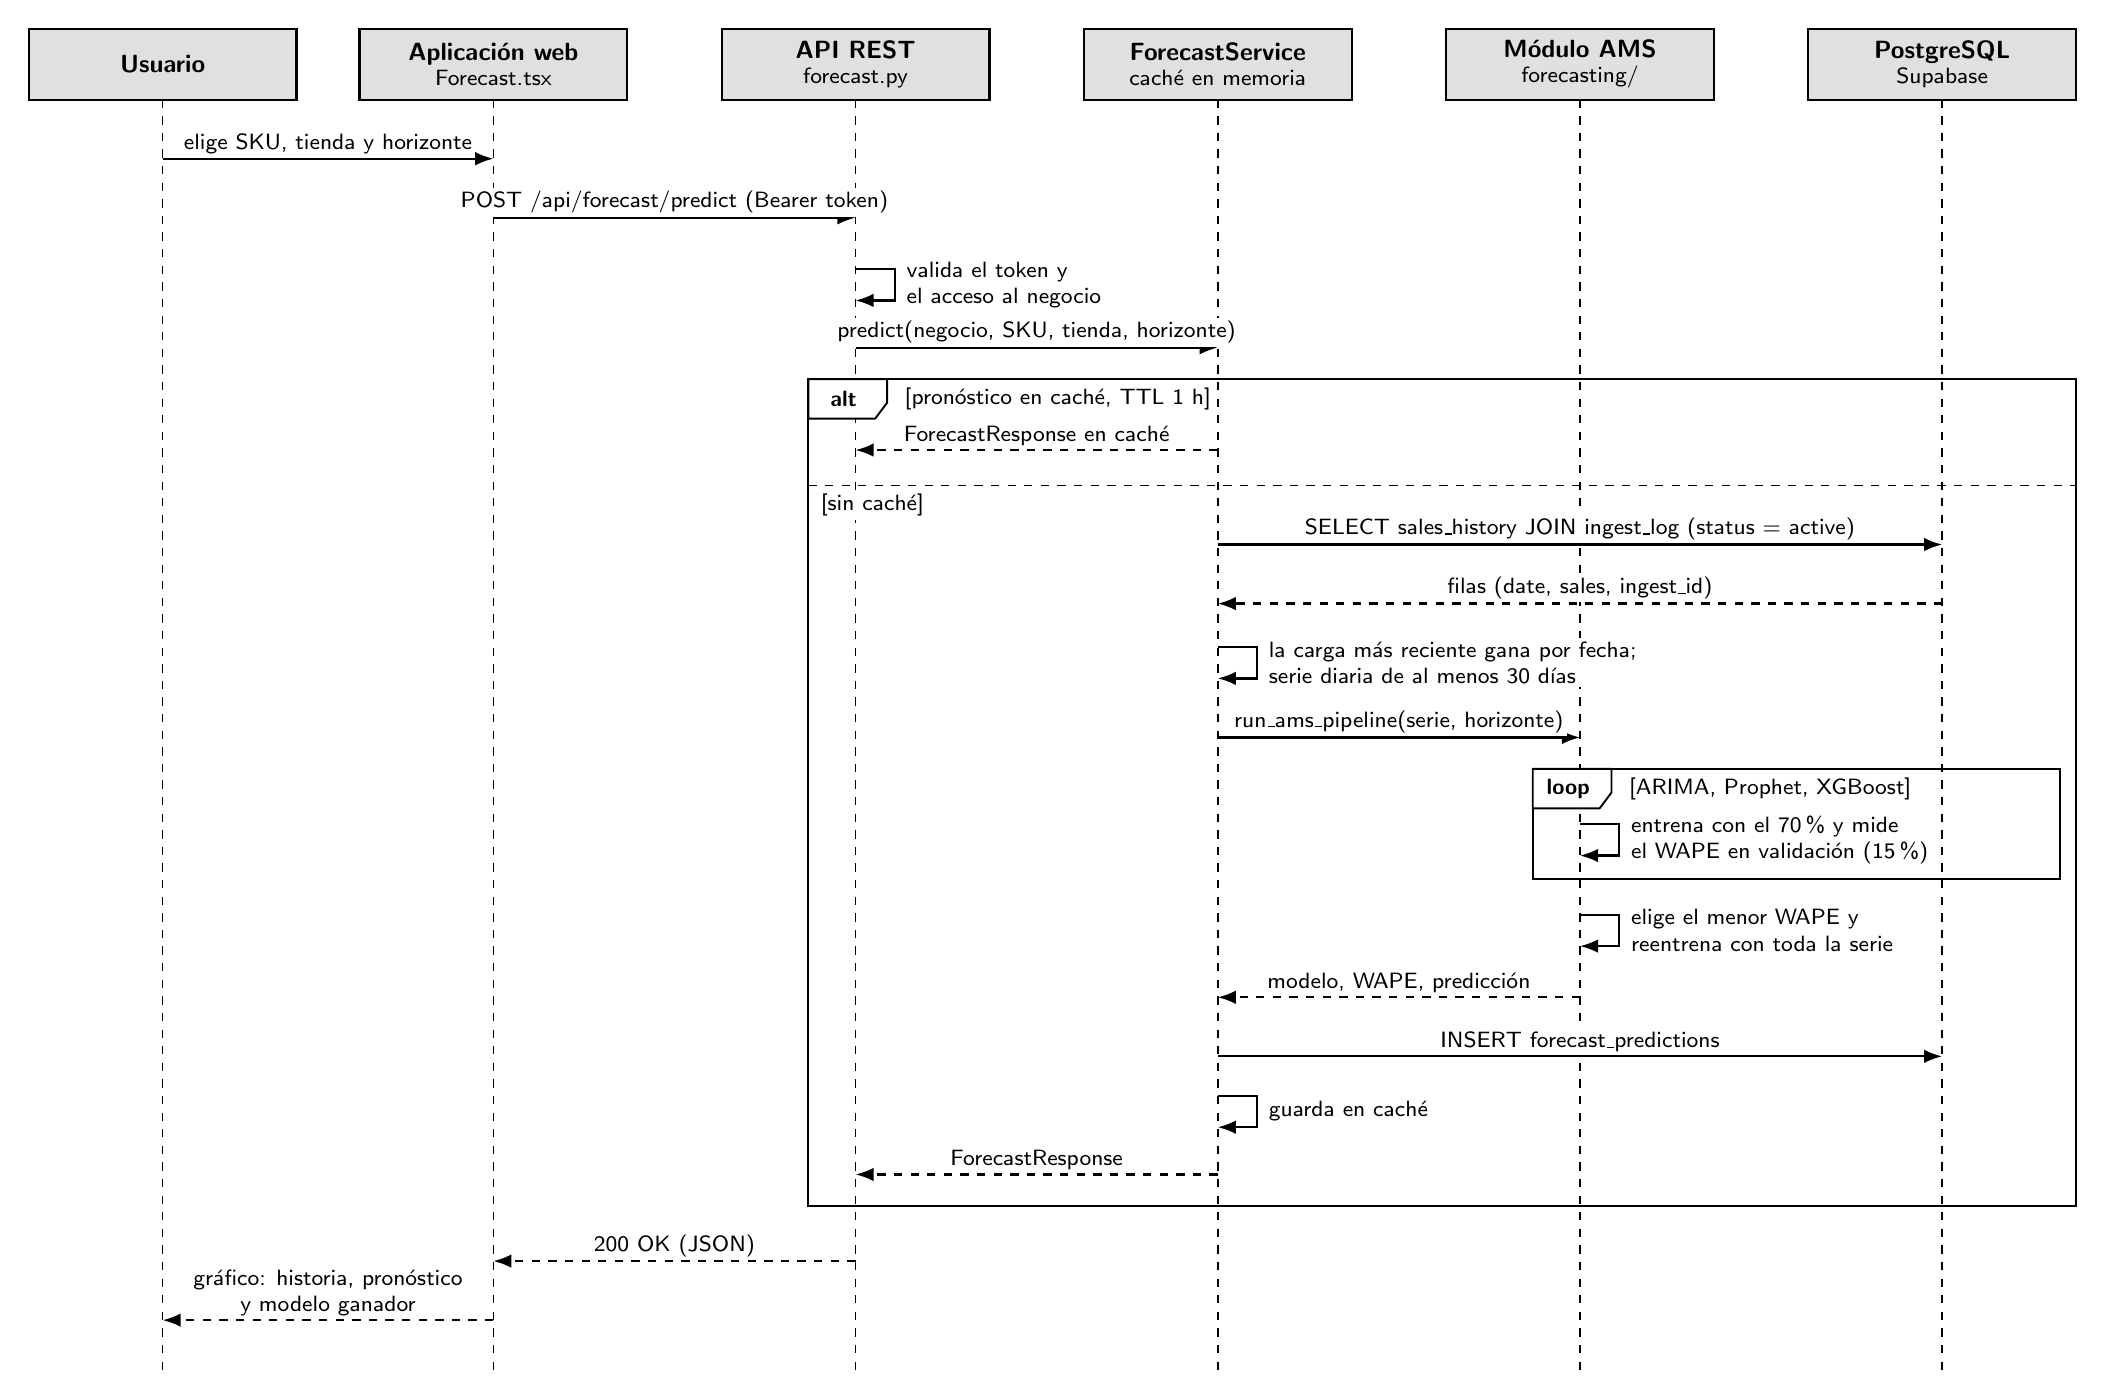
\begin{tikzpicture}[font=\sffamily]

\node[head] at (\xU,0) {Usuario};
\node[head] at (\xA,0) {Aplicación web\\[-2pt]{\footnotesize\mdseries Forecast.tsx}};
\node[head] at (\xB,0) {API REST\\[-2pt]{\footnotesize\mdseries forecast.py}};
\node[head] at (\xS,0) {ForecastService\\[-2pt]{\footnotesize\mdseries caché en memoria}};
\node[head] at (\xM,0) {Módulo AMS\\[-2pt]{\footnotesize\mdseries forecasting/}};
\node[head] at (\xD,0) {PostgreSQL\\[-2pt]{\footnotesize\mdseries Supabase}};
\foreach \x in {\xU,\xA,\xB,\xS,\xM,\xD} \draw[dashed, line width=0.6pt] (\x,-0.45) -- (\x,-16.6);

\msg{\xU}{\xA}{-1.2}{elige SKU, tienda y horizonte}
\msg{\xA}{\xB}{-1.95}{POST /api/forecast/predict (Bearer token)}
\self{\xB}{-2.6}{valida el token y\\el acceso al negocio}
\msg{\xB}{\xS}{-3.6}{predict(negocio, SKU, tienda, horizonte)}

\frag{8.2}{-4.0}{24.3}{-14.5}{alt}{[pronóstico en caché, TTL 1 h]}
\ret{\xS}{\xB}{-4.9}{ForecastResponse en caché}
\els{8.2}{-5.35}{24.3}{[sin caché]}
\msg{\xS}{\xD}{-6.1}{SELECT sales\_history JOIN ingest\_log (status = active)}
\ret{\xD}{\xS}{-6.85}{filas (date, sales, ingest\_id)}
\self{\xS}{-7.4}{la carga más reciente gana por fecha;\\serie diaria de al menos 30 días}
\msg{\xS}{\xM}{-8.55}{run\_ams\_pipeline(serie, horizonte)}
\frag{17.4}{-8.95}{24.1}{-10.35}{loop}{[ARIMA, Prophet, XGBoost]}
\self{\xM}{-9.65}{entrena con el 70\,\% y mide\\el WAPE en validación (15\,\%)}
\self{\xM}{-10.8}{elige el menor WAPE y\\reentrena con toda la serie}
\ret{\xM}{\xS}{-11.85}{modelo, WAPE, predicción}
\msg{\xS}{\xD}{-12.6}{INSERT forecast\_predictions}
\self{\xS}{-13.1}{guarda en caché}
\ret{\xS}{\xB}{-14.1}{ForecastResponse}

\ret{\xB}{\xA}{-15.2}{200 OK (JSON)}
\ret{\xA}{\xU}{-15.95}{gráfico: historia, pronóstico\\y modelo ganador}

\end{tikzpicture}
\end{document}
